\documentclass{article}
\usepackage[utf8]{inputenc}
\usepackage[T1]{fontenc}
\usepackage{natbib}
\usepackage{hyperref}
\usepackage{graphicx} % Required for inserting images
\usepackage{listings}
\usepackage{xcolor}
\usepackage{amsmath}
\usepackage{algorithm}
\usepackage{algorithmic}
\usepackage{algpseudocode}

\lstset{
    backgroundcolor=\color{lightgray}, % background color
    basicstyle=\footnotesize\ttfamily, % font size and type
    breaklines=true, % enables line breaking
    frame=single, % adds a frame around the code
    numbers=none, % disable line numbers
    keywordstyle=\color{blue}, % keyword color
    commentstyle=\color{green}, % comment color
    stringstyle=\color{red}, % string color
    linewidth=1.2\textwidth, % adjusts the width of the code block
    xleftmargin=1em, % left margin for the code block
    xrightmargin=1em % right margin for the code block
}


\title{PMPH group project: Sorting on GPUs}
\author{Mathias Heldbo (tzc182), Rasmus Gabelgaard Nielsen (ncg106) \\ and Hans Peter Lyngsøe (pvr448)}
\date{November 2024}

\begin{document}

\maketitle

\section{The radix sort algorithm }
In order to gain an understanding of radix sort, the sequential implementation will be discussed, and then a discussion of parallelization using basic blocks. 
\begin{itemize}
\item Radix sort
The basic idea of radix sort is to sort an integer into digits consisting of r bits. Then the list is sorted for each digit until all digits have been traversed and the list is fully sorted. The main assumption of radix sort is that all integers in the input list can be split into digits
\item Radix sort sequential:
The sequential implementation iterates through the digits, r bits at a time, a standard implementation is 1 bit at a time, but more is more efficient. Each digit m, has r bits, such that $m = 2^r$. Radix sort works by performing a counting sort on each set of digits, until all digits have been traversed. Counting sort follows the following syntax: 
\begin{figure} [H]
    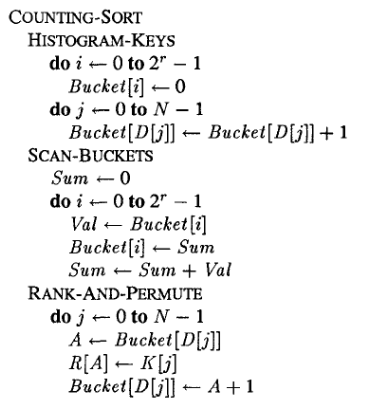
\includegraphics[width=0.5\linewidth]{count_sort.PNG}
    \caption{Counting Sort \citep{zagharadixvector}}
    \label{fig:enter-label}
\end{figure}.

Where Histogram-Keys counts the number of elements in a bucket for each unique digit. Scan-Buckets, scan the buckets and returns the position at which the first element of a subset having a certain digit is to be placed, that is, the offset. Finally, Rank-and-permute matches the digit value with the bucket offset and iterates through each "sub bucket" to order the elements by their digit. After this, counting sort is repeated on each subset of digits until the whole list is sorted.  
\item For parallelization of radix sort, similar ideas are used, however, there a few key differences. One such method is discussed in \citep{zagharadixvector}. With p processors, the input list is split into p sub-lists for each processor to work on. Each processor performs Histogram-keys locally to create local histograms, then scan buckets is run globally to calculate the global offset, Rank and Permute can then be performed locally and written to global memory as Rank and Permute takes in the offset, and therefore doesn't overwrite the work done by other processors \citep{zagharadixvector}.

Let us now consider a very simple parallel radix sort implementation going through 1 bit at a time, for 32 bit integers using basic blocks, and let us consider the example of
$$\begin{bmatrix} 1, 4, 2, 3\end{bmatrix}$$
with a bit representation of: 
$$\begin{bmatrix} 001, 100, 010, 011\end{bmatrix}$$
Please bear in mind that this implementation is a very simplified parallel radix sort implementation in Futhark using basic blocks such as map, scan, reduce and scatter. Due to its syntax, Futhark automatically distributes the processes depending on available processors, however, better approaches are discussed in part 2. 
\begin{lstlisting}

-- xs = [1,4,2,3] in integer format
-- xs = [001, 100, 010, 011] in bit format 
def radix_bit [n] 't (f: t -> u32) (xs: [n]t) (b: i32): [n]t =
(1)    let bits = map(\x -> (i32.u32 (f x >> u32.i32 b )) & 1) xs -- [1, 0, 0, 1], D = O(1), W = O(n)
(2)    let bits_neg = map (1-) bits                               -- [0, 1, 1, 0], D = O(1), W = O(n)
(3)    let offs = reduce (+) 0 bits_neg                           -- 2,            D = O(log n), W = O(n)
(4)    let idxs0 = map2 (*) bits_neg (scan (+) 0 bits_neg)        -- [0, 1, 2, 0], D = O(log n), W = O(n)
(5)    let idxs1 = map2 (*) bits (map (+offs) (scan (+) 0 bits))  -- [3, 0, 0, 4], D = O(log n), W = O(n)
(6)    let idxs2 = map2 (+) idxs0 idxs1                           -- [3, 1, 2, 4], D = O(1), W = O(n)
(7)    let idxs = map (\x -> x-1) idxs2                           -- [2, 0, 1, 3], D = O(1), W = O(n)
(8)    let xs' = scatter (copy xs) idxs xs                        -- [4, 2, 1, 3], D = O(1), W = O(n)
       -- in terms of the bit in question, it becomes        [100, 010, 001, 011]
(9)    in xs'                                                                   -- D = O(log n), W = O(n)

def radix [n] 't (f: t -> u32) (xs: [n]t): [n]t = 
(10)    loop xs for i < 32 do radix_bit f xs i                     -- D = O(log n), W = O(n)
\end{lstlisting}

This implementation is from \href{https://futhark-lang.org/examples/radix-sort-key.html}{radix-sort-key (futhark-lang.org)}, and applied to each bit of 32 bit unsigned integers, as radix sort requires each digit to be in the range of 0 to m-1. The radix\_bit part of the algorithm takes in a bit. The bits are stored in bits (1), bits\_neg (2) contains the bits converted to their compliment, offs (3), get the offsets of the bits by calculating how many 0 bits there are, which is what bits\_neg is used for. Idxs0 (4) finds the indices of elements with a bit of 0, while idxs1 (5) finds the indices of elements with a bit of 1, and idxs2 (6) concatenate those two lists. Indexes are then stored in idxs (7) assuming zero indexing, by subtracting 1 from every index. Then scatter (8) is used to distribute the elements to their corresponding location.
\\
Let us now consider the work depth complexity, for a list of length n, the work and depth complexity is written next to the code, where scan and reduce both have a depth complexity of O(log n), and all lines have O(n) work complexity, as they traverse n elements. While this work depth complexity might seem good on paper, this is a best case scenario, in which we always have n processors. More advanced methods deal with the distribution of the workload in a fashion more suited to the GPU, and this improving the overall speed and efficiency of the algorithm. 
\end{itemize}

\section{Fast parallel radix sort}

Although \citep{zagharadixvector} was great at the time, our literature search provided several higher performing parallel radix sorts. The first implementation by Satish et. al. provides a significant speed up from previous methods using the following ground principles and distributing 4 bit digits per thread, 
\begin{figure} [H]
    \centering
    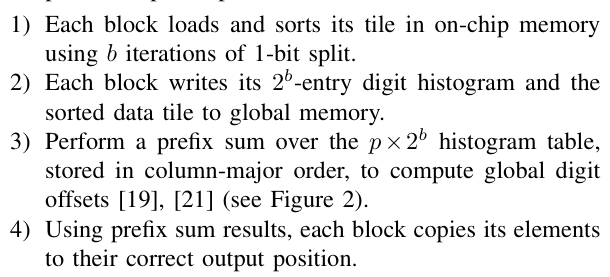
\includegraphics[width=\linewidth]{satish.PNG}
    \caption{Satish steps \citep{satish}}
    \label{fig:enter-label}
\end{figure}.
They also proposed parallel local radix counting and pre-sorting as well as global radix ranking and coalesced global shuffling\citep{satish}Building off these concepts, Ha. et. al proposed two improvements, implicit counting and a mixed-data structure with 4 elements, that is 2-bit digits.
\begin{itemize}
\item Implicit counting \\
Uses bit shifting to create a 32-bit register for radix value 0, 1 and 2. With the count of 0 assigned to bits from 0 to 9, the count of 1 assigned to bit values from 10-19, and the count of 2 assigned to bits from 20-29. The implicit count is: $$impl_{cnt} = cnt_0 + (cnt_1 \ll 10) + (cnt_2 \ll 20)$$
The implicit value is: 
$$impl_{val} = (val \lt  3) \ll (10 \cdot val)$$
$impl_{cnt}$ is calculated by incrementing by the $impl_{val}$:
$$impl_{cnt} = impl_{cnt} + impl_{val}$$
The count is retrieved by: 
$$cnt\begin{bmatrix}val\end{bmatrix} = impl_{cnt} \gg (10 \cdot val) $$
and the fourth counting value is retrieved by:
$$cnt\begin{bmatrix} 3 \end{bmatrix} = idx - cnt\begin{bmatrix} 0 \end{bmatrix} - cnt\begin{bmatrix} 1 \end{bmatrix} - cnt\begin{bmatrix} 2 \end{bmatrix}$$
Thus implicit counting reduces the count operations from 4 in Satish. et. al to 2. 
\item Mixed-data structure \\

\begin{figure} [H]
    \centering
    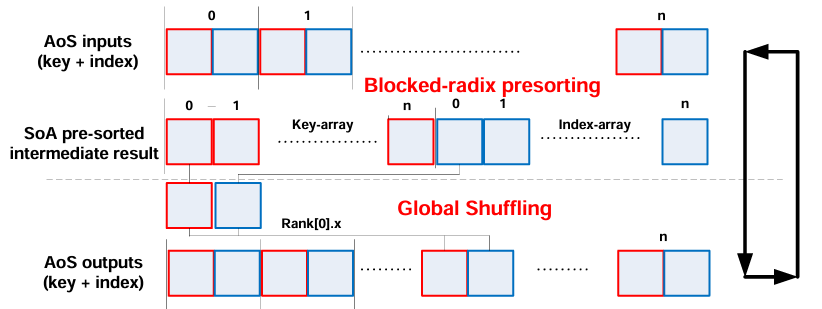
\includegraphics[width=\linewidth]{mixed-data.PNG}
    \caption{Mixed data method \citep{ha2010implicit}}
    \label{fig:enter-label}
\end{figure}.
Ha. et. al's hybrid data structure uses AoS and SoA, which reduces suboptimal coalesced scattering effects, and requires only one shuffle pass on the pre sorting data due to the structure \citep{ha2010implicit} 
\\
We have decided to attempt to implement the Ha. et. al algorithm
\item Pseudocode



\end{itemize}
\begin{lstlisting}
1. Initialize data structures:
   - Load input keys and values.
     * Work: O(n), Depth: O(1)
   - Assuming the input is integers we can map from 32 to 24 bit by:
   - Determine [a,b] using reduce
     * Work: O(n), Depth: O(log n)
   - Map input values from a, b to [0, b-a]
     * Work: O(n), Depth: O(1)
     
2. Iterate through bit shifts:
   For each bit shift (e.g., 4 bits per pass):
     - Map the current bit shift to all elements.
       * Work: O(n), Depth: O(1)
     - Create an array of structures `AoS` by associating each element's index and key.
       * Work: O(n), Depth: O(1)

3. Local counting and presorting (within each block):
   - For each block of block size B * 4 elements:
     - Compute implicit counts:
       * Work: O(B*4)  per block, total O(n), Depth: O(log B*4)

     - Calculate the local rank for each element in the block using **exclusive scan** on the histogram:
       * Work: O(B*4) per block, total O(n), Depth: O(log B*4)

     - Scatter locally (pre sort):
       * Work: O(B) per block, total O(n), Depth: O(1)

4. Global ranking and offset calculation:
   - Compute global offsets using **prefix sum** (scan) across all local histograms:
     * Work: O(P) = O(n/(B))
     * Depth: O(log P) = O(log n/(B))

   - Adjust local ranks by adding block offsets:
     * Work: O(n), Depth: O(1)

5. Global shuffling and final scatter:
   - Scatter elements globally using computed global offsets:
     * Work: O(n), Depth: O(log B)

6. Repeat until all bits are processed.
   - Number of passes depends on bit width (e.g., for 24-bit keys (mapping from 32 to 24) with 2 bits (4 elements) per pass, we need 16 passes).
   - Total:
     * Work: O(n * #passes), Depth: O(#passes * (log B + log P) = O(#passes * (log B + log (n/B)))
\end{lstlisting}

Additionally, the algorithm has bank conflict-free access, storing in different arrays to avoid concurrent access, 
Mapping of integers from [a,b to 0, b-a] for integers, and floats by mapping from [a,b] to [0.5, 1] to change from 32 bit to 24 bit. 30\% performance increase. It is an approximation but it is precise enough.

\section{In depth cuda implementation}
We split our implementation of the parallel radix sort on cuda into four main kernels:
\begin{itemize}
    \item Histogram kernel
    \item Transpose kernel
    \item Scan kernel
    \item A final rank and permute kernel
\end{itemize}

We follow the possible good values recommended, thus $Q = 22, lgH = 8, H = 256, B = 256$.

\subsection{Histogram kernel}
The parallel cuda-implementation of the histogram processes $Q$ elements per thread. We decided to use shared memory while processing the histogram, as otherwise we would have to access global memory many times, which is slower than first using shared memory, and then writing the final histogram to global memory.

Unfortunately we use atomic adds for incrementing our histogram buckets. This is done $Q$ times per thread, which is not ideal, as atomic adds impacts performance negatively, which likely affects our results as seen in the last section.

Notably for the histogram we sort each element based on each bit, instead of the regular approach of sorting by each digit. This approach is both more memory efficient and faster.  

\subsection{Transpose kernel}

The transpose kernel is relatively simple and is heavily inspired by the one presented in the week 2 assignment. This transpose kernel use a tiled approach where we use memory coalescing to ensure better performance. We transpose in blocks of size 256, thus we use tile size of 16x16, which also means we can leverage shared memory before they are written to global to maximize performance.

We use this transpose kernel twice, once before scanning and then again after scanning, as this gives us back the original histogram shape. Note that the array we transpose is simply a 1d-array, so we have to keep that in mind and use the correct width and height to represent our matrix correctly. Consequently, we ensure we access the the 1d array with a stride of 1.

\subsection{Scan kernel}
The scan kernel is called on the transposed matrix to gain indices for the rand-and-permute kernel. We use inclusive scan on our histogram

%TODO Write more for this

\subsection{Rank-and-permute kernel}
The rank-and-permute kernel (the final kernel) starts by copying our global scanned matrix into shared memory and then register memory, which allows for faster access to the memory, as we have many reads and writes, and should also allow for coalesced memory access. Then in a loop of size lgH we apply two-way partition for Q elements in our current block.

%TODO Write more here

After the two-way partition we need to copy from our register memory back to global memory. This is done by copying the original and scanned histogram from global to shared memory. Then we can scan the original histogram in order to obtain the correct indices for our elements in each block. Finally based on these indices we can now write all elements processed for each block back to the the final global array, which will be our sorted array.

\subsection{Sorting the whole array}
In order to sort the entire array, we apply the above kernels for each bit in a loop. This means our sorting algorithm first takes in a completely unsorted array, then applies all the kernels to it. After the rank-and-permute kernel, we overwrite the input array we gave to the histogram and build a new array on the result of the rank-and-permute kernel. This process is then repeated, where the histogram is build on the rank-and-permute output, for however many bits our elements in our array have. As we are using 32 bit numbers, it means we launch the kernels 32 times to obtain a fully sorted array. Consequently, this can have an effect on the performance of our sorting and some papers like \cite{p} suggest that for instead of building a histogram for each bit, it was more beneficial if we processed four bits at a time, which would lead to only launching the kernels 8 times for 32 bit number. 

\section{Performance evaluation}
We benchmarked cuda, futhark and our own implementation. The results were the following:
%TODO...

\subsection{Discussion of results}

\subsection{Suggestions for improving our cub implementation}

\bibliographystyle{plainnat}
\bibliography{references}

\end{document}
